\section{Background}
\label{sec:background}
We first briefly overview the issues in designing an pub/sub-based middleware for WSN.

\subsection{Events and Event Types}
In our event model, each event is a list of attributes which are the actual data obtained from the sensor networks \cite{lowlevelnaming}. The detected events can be filtered with subscriptions. There are mainly three types of subscriptions: content-based, topic-based and type-based \cite{facespubsub}. In PSWare, we use type-based subscription because composite events can be more easily defined by specifying their types and the corresponding filters \cite{siena}.

Events can be primitive or composite based on their types. Primitive events are those that can be detected by individual sensor nodes directly while Composite events are those that can be detected when some other events satisfy certain relations among them. These relations may be temporal or spatial and may be expressed as operators. 

Events together with their relations can be represented as a directed acyclic graph where each node represents an event and the each edge represents a relation. Figure \ref{fig:eventhierarchy} shows an example of such a graph. The nodes with 0 indegree represent primitive events. The rest of the nodes represent composite events. The event which has 0 outdegree is the subscribed event.

\begin{figure}
\centering
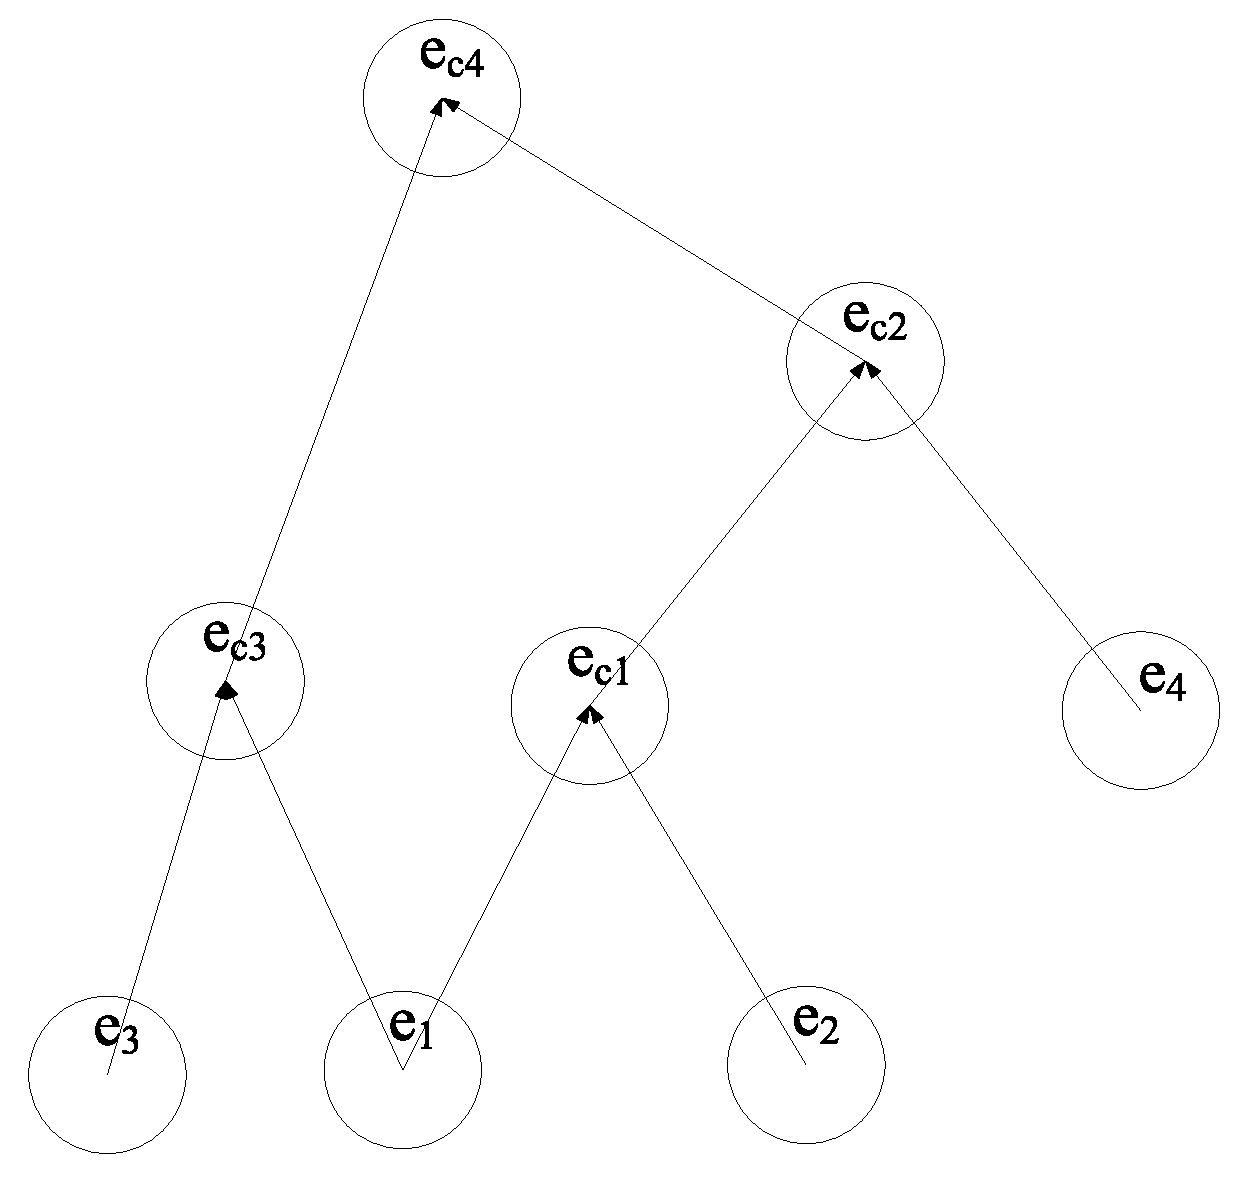
\includegraphics[width=.3\textwidth]{eventhierarchy}
\caption{Event hierarchy}
\label{fig:eventhierarchy}
\end{figure}

Once the subscriptions are defined, it will be disseminated into the network so that sensor nodes can start to monitor. The sensor nodes collect data in rounds. In each round, the collected data will be matched against the subscription. If an event is found to match the subscribed event type, it will be delivered to the sink to notify the subscriber.

\subsection{Event Detection and Detection Cost}
Events can be detected with different strategies based their types and relations. In this paper, we mainly consider message cost as event detection cost. Furthermore, since primitive event can be detected by individual sensor nodes, we mainly consider the composite event detection cost in this paper.

In general, if a composite event is detected based on two sub-events \(e_1\) and \(e_2\) as shown in Figure \ref{fig:event-detection2} then the cost for detecting the composite event will be the cost for detecting each individual events together with the cost for delivering the event detection results to the event detector. An event detector here is simply a node responsible for detecting composite events.

\begin{figure}
\centering
\subfloat[Basic composite event detection]{\label{fig:event-detection2}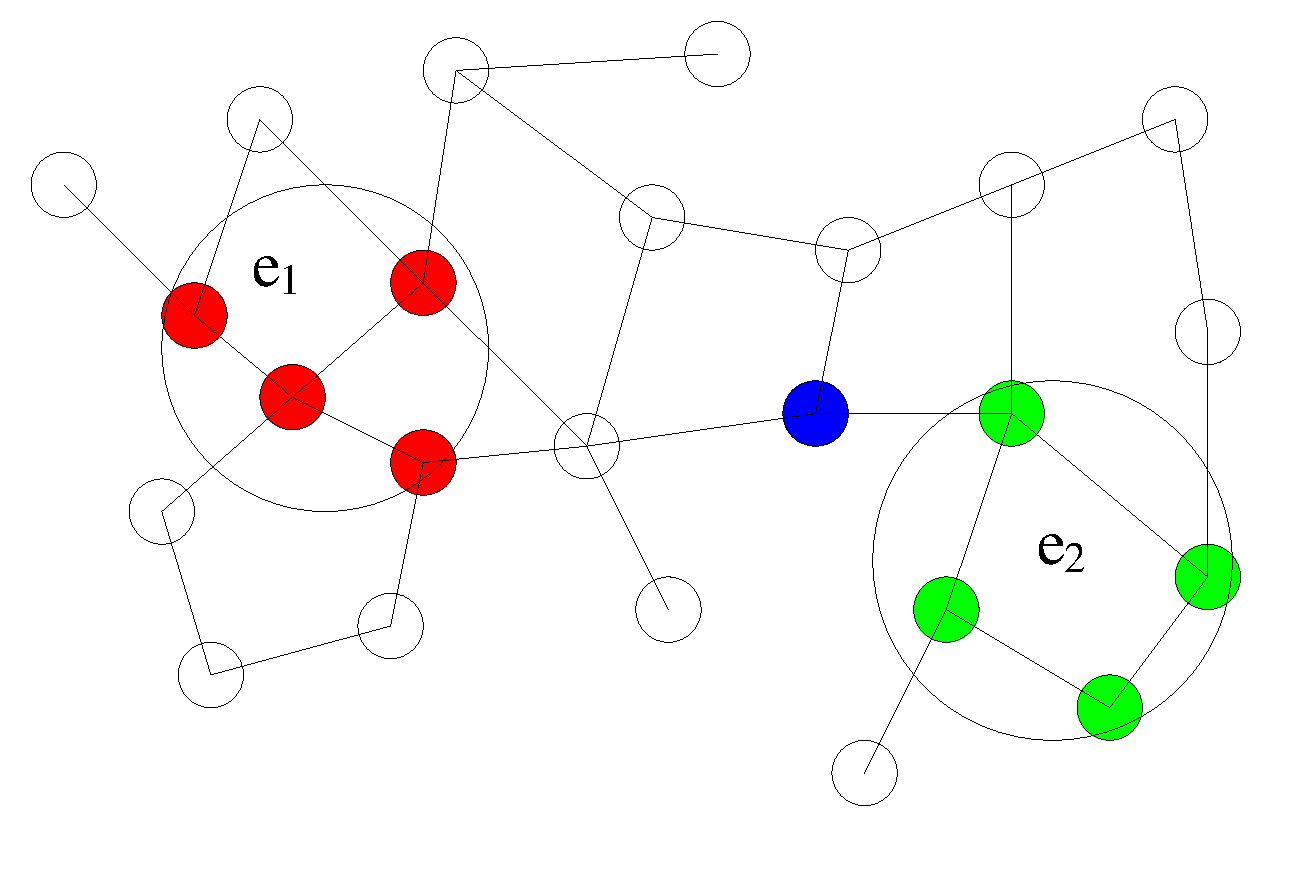
\includegraphics[width=.3\textwidth]{event-detection2}}
\qquad
\subfloat[Composite event detection using event probability]{\label{fig:event-detection3}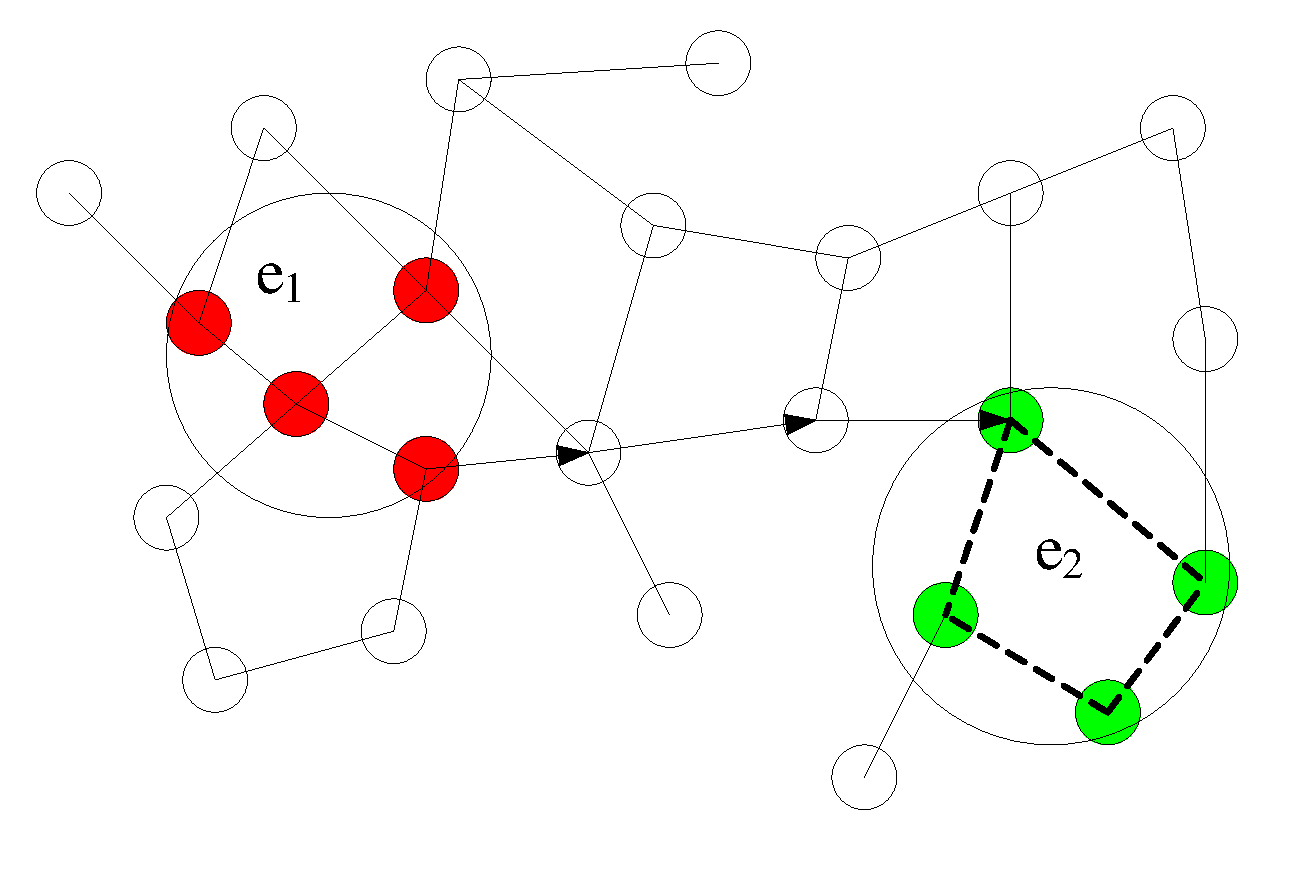
\includegraphics[width=.3\textwidth]{event-detection3}}
\caption{Composite event detection}
\label{fig:event-detection}
\end{figure}

Sometimes the events may have dependency and certain events must happen before others. In this case, we don't need to make all sensor nodes monitor the events at all the time. Instead, some nodes may firstly put to sleep mode and then be waken up when other events occur. For example, as shown in Figure \ref{fig:event-detection3}, if we have two events \(e_1\) and \(e_2\) which have a relation such that the composite event happens only when both events have been successfully detected. If \(e_2\) and \(e_1\) need to satisfy a relation such that \(e_2\) happens after \(e_1\). Then originally the nodes responsible for monitoring \(e_2\) may be put to sleep mode. After \(e_1\) has successfully been detected, a message can be forwarded to the nodes responsible for detecting \(e_2\) and wake them up. In this way, we can further reduce the energy cost because \(e_2\) doesn't have to be monitored if \(e_1\) doesn't occur.
